\documentclass{sig-alternate}

\usepackage{xcolor}
\usepackage{lipsum}
\usepackage{url}

\usepackage{balance}
\usepackage{microtype}

\DeclareSymbolFont{extraup}{U}{zavm}{m}{n}
\DeclareMathSymbol{\varheart}{\mathalpha}{extraup}{86}
\DeclareMathSymbol{\vardiamond}{\mathalpha}{extraup}{87}

\usepackage{booktabs}

% \usepackage[pdftex]{graphicx}
\graphicspath{{./figures/}}

\begin{document}

\toappear{}

%
% --- Author Metadata here ---
%\conferenceinfo{ESEC/FSE}{'15 Bergamo, Italy}
%\CopyrightYear{2015} % Allows default copyright year (20XX) to be over-ridden - IF NEED BE.
%\crdata{0-12345-67-8/90/01}  % Allows default copyright data (0-89791-88-6/97/05) to be over-ridden - IF NEED BE.
% --- End of Author Metadata ---

\title{I \scalebox{1.7}{\color{red} $\varheart$} Hacker News}
\subtitle{Expanding Qualitative Research Findings by Analyzing Social News Websites}

\numberofauthors{3}

\author{
\alignauthor
Titus Barik\\
       \affaddr{ABB Corporate Research}\\
       \affaddr{Raleigh, North Carolina, USA}\\      
       \email{titus.barik@us.abb.com}
\alignauthor
Brittany Johnson\\
       \affaddr{NC State University}\\
       \affaddr{Raleigh, North Carolina, USA}\\      
       \email{bijohnso@ncsu.edu}
\alignauthor
Emerson Murphy-Hill\\
\affaddr{NC State University}\\
\affaddr{Raleigh, North Carolina, USA}\\      
\email{emerson@csc.ncsu.edu}}

% There's nothing stopping you putting the seventh, eighth, etc.
% author on the opening page (as the 'third row') but we ask,
% for aesthetic reasons that you place these 'additional authors'
% in the \additional authors block, viz.
\additionalauthors{Additional authors: John Smith (The Th{\o}rv{\"a}ld Group,
email: {\texttt{jsmith@affiliation.org}}) and Julius P.~Kumquat
(The Kumquat Consortium, email: {\texttt{jpkumquat@consortium.net}}).}
\date{30 July 1999}
% Just remember to make sure that the TOTAL number of authors
% is the number that will appear on the first page PLUS the
% number that will appear in the \additionalauthors section.

\maketitle
\begin{abstract}
Grounded theory is an important research method in empirical software engineering, but it is also time consuming, tedious, and complex. This makes it difficult for researchers to assess if threats, such as missing themes or sample bias, have inadvertently materialized. To assess such threats, our new idea is that we can automatically extract knowledge from social news websites, such as Hacker News, to easily replicate existing grounded theory research --- and then compare the results. We conduct a replication study on static analysis tool adoption using Hacker News. We confirm that even a basic replication and analysis using social news websites can offer additional insights to existing themes in studies, while also identifying new themes. For example, we identified that security was not a theme discovered in the original study on tool adoption. As a long-term vision, we consider techniques from the discipline of knowledge discovery to make this replication process more automatic.
\end{abstract}

% TODO(tbarik): Fix ACM classification system.
% A category with the (minimum) three required fields
\category{D.2.10}{Software Engineering}{Design}
\category{I.1.m}{Computing Methodologies}{Miscellaneous}
%A category including the fourth, optional field follows...


% \terms{Design, Human Factors}

\keywords{Grounded theory, computer-mediated discourse, Hacker News, representativeness, theoretical saturation}

\section{The Problem}

Because human activities play a central role in software development, many research methods borrow from traditional empirical disciplines that study human behavior, such as sociology or anthropology~\cite{Easterbrook2008}. Motivated by the desire to understand the experiences of actual software practitioners, \textit{grounded theory} is one such empirical research method that has been applied to the study of software development~\cite{Adolph2011}.

While researchers disagree on the ``correct'' execution of grounded theory practices~\cite{Suddaby2006}, the basic tenet of grounded theory is that insights are generated from collected data, which are then \textit{coded}, or categorized, in a bottom-up fashion to form a theory. In essence, grounded theory is ``a method for discovering the real problem that exists for the participants in a substantive area rather than what professional researchers may believe is their problem''~\cite{Adolph2008}. As Brown notes, ``the mandate of grounded theory is to develop theories based on people's lived experiences rather than on proving or disproving existing theories''~\cite{brown2012daring}. Put another way, grounded theory provides a systematic and formal approach to ask software practitioners: ``What's going on here?''

Unfortunately, grounded theory is also time consuming, tedious, and complex~\cite{Olson2014} --- and like all research methods, has its own requirements, affordances, and limitations. For technical communities who engage largely in quantitative research, three of these requirements cause much angst. First, grounded theory requires that we use \textit{theoretical sampling}, that is, sampling to maximize the diversity of the individuals rather than the size of the sample. Second, the method requires us to reach \textit{theoretical saturation}, or sampling to the point in which no new data appear --- that is, a ``stop-rule''. Third, replication, or other forms of data triangulation, is the recommendation for \textit{transferability} of the theory.

A significant threat is that the grounded theory guidelines for these requirements are presented under some ideal model of unbounded time and infinite constraints --- in practice, however, this model is unsatisfiable~\cite{Mason2010}. For example, sampling may be constrained by physical and geographic factors, which in turn in reduce diversity and trigger theoretical saturation prematurely. And despite its importance, the time consuming nature of grounded theory studies, as well as finite budgets, means that the likelihood that one will actually a conduct a replication is rare~\cite{Shull2008b}.

This confluence of these threats makes it difficult for researchers to assess the quality of the \textit{theory} in grounded theory. To address this challenge, this paper investigates the suitability of using posted comments in social news websites as a source of knowledge to mitigate these threats. In the longer term, we propose techniques from knowledge discovery and databases (KDD) and adapt them to grounded theory processes to allow for automatic replication.

\section{What is the New Idea?}

\begin{figure}
\centering
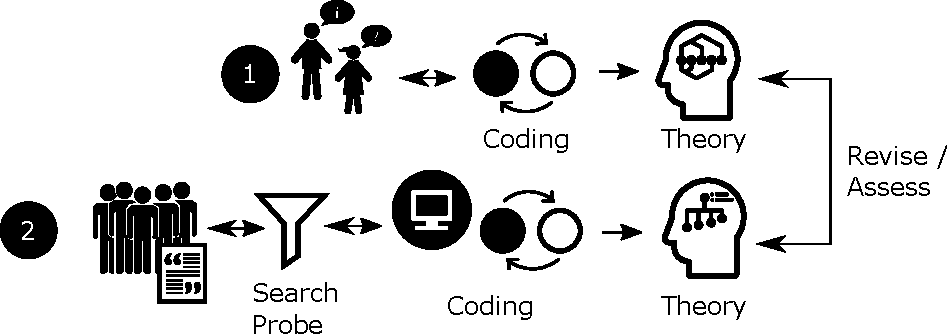
\includegraphics[width=\linewidth]{concept}
\caption{A comparison of the method for (1) a classical empirical studies and (2) a social news website study. In this scenario, a replication study (2) is conducted using Hacker News. Filtering and topic analysis can be automatically or semi-automatically performed. The output of this replication can then be compared with the original empirical study. The double-arrows reflect that grounded theory is not a step-by-step procedure, but an iterative way of thinking about data.\label{fig:concept}}
\end{figure}

Our new idea is that we can automatically extract knowledge from comments on social news websites, such as Reddit\footnote{\url{https://www.reddit.com/}}, Slashdot\footnote{\url{http://www.slashdot.org/}}, and Hacker News\footnote{\url{https://news.ycombinator.com/}}, to obtain software developer experiences and beliefs for the types of topics that would typically be encountered or asked in grounded theory research. Importantly, unlike surveys or interviews, which require active recruitment to obtain such information, our approach exploits latent knowledge from historical conversations about such topics.

For example, in a technical community, a software engineering researcher might ask the research questions, ``Why don't developers use static analysis tools?''~\cite{Johnson2013a}, ``What makes a great software engineer?''~\cite{Li2015}, or ``What are the practices of agile teams?''~\cite{Hoda2011}. We postulate that when such questions are applied against an appropriate social news website, the quality of the results are comparable to the results obtained from empirical research approaches with similar output artifacts --- such as those obtained in interviews.

The implementation of our idea can be used to enhance software engineering research in several ways.  For example, consider Fig.~\ref{fig:concept}-1, in which an empirical researcher has already conducted a grounded theory study in which he has interviewed participants, coded the responses, and generated a theory. However, the researcher is concerned about the use of students subjects in the study. In our approach (Fig~\ref{fig:concept}-2), the researcher can simply submit a search probe to a social news website using the research question. Because these websites catalog a diverse set of stories, comments relevant to the researcher's probe are likely to exist in the dataset. Using analysis software that implements our technique, the software will extract relevant comments, use machine learning to automatically or semi-automatically code and categorize the responses, and allow the researcher to evaluate the generated theory against the theory derived from the empirical study.

Prior to conducting an in-person empirical study, a researcher may use our technique as a pilot to quickly identify interesting responses to their proposed software-related research question. The researcher can use these results as a tool to guide their coding strategies, by having a set of seed responses. Finally, given a diverse enough dataset, we may also be able to treat this technique as a first-class, stand-alone method for conducting grounded theory research.

% TODO(tbarik): Talk about the example.

\section{Why Is It New?}

Grounded theory practices have been successfully applied to online software engineering communities to extract useful knowledge.
For example, in addition to quantitative analysis, Vendome and colleagues conducted grounded theory on commit notes and issue tracker discussions in GitHub to identify why developers change software licenses~\cite{Vendome2015}. Tsay and colleagues used grounded theory in GitHub to understand how project members evaluate and discuss contributions to the project~\cite{Tsay2014}. Through StackOverflow\footnote{\url{http://stackoverflow.com/}}, Nasehi and colleagues used grounded theory on user posts to identify characteristics of effective code examples~\cite{Nasehi2012}.

However, we are unaware of any research in software engineering that has explicitly attempted to use social news websites to answer multiple grounded theory questions through a generalized technique. Nor are we aware of any efforts to replicate grounded theory studies using online communities.

Our own grounded theory work in understanding why developers use or do not use static analysis tools\footnote{Static analysis tools provide analysis on source code, without actually executing the program. They are commonly used for finding defects in code.} is the catalyst for the new idea described in this paper~\cite{Johnson2013a}. Our interest in this topic is motivated by the experiences in our research lab regarding the cost of conducting grounded theory studies, as well as our desire to increase our own confidence in these types of studies. Thus, our static analysis adoption work is the basis for this paper.

\section{A Proof-of-Concept Replication of Tool Adoption}

In this section, we conduct a proof-of-concept replication study using our proposed idea. We perform replication to our previous work on why developers don't use static analysis tools~\cite{Johnson2013a}. In this original study, we used 20 participants with industry experience. The study session consisted of a semi-structured interview, followed by an interactive interview. A grounded theory analysis was conducted on the transcripts from those interviews.

For purposes of space, we replicate only the primary question from the study, ``What reasons do developers have for using or not using static analysis tools to find bugs?'' In this replication, we use Hacker News as the underlying data source. 

We chose Hacker News for this replication for several reasons. First, it has active discussions, with over 7.5 million comments. Second, Hacker News attracts a technical audience, which means responses to grounded theory questions relating to software engineering are abundant. Third, Hacker News has strict moderation guidelines, as well as comment ranking through a points system, both of which help to enhance the overall quality of comments.

Using Hacker News, we validate our concept through three research questions:

\begin{description}
\item[RQ1] Is there enough knowledge available within Hacker News to replicate our study?
\item[RQ2] Are there codes (that is, themes) that we obtain from Hacker News that we failed to identify in our study?
\item[RQ3] Can knowledge extraction be conducted automatically?
\end{description}

% We use our prior work, based on grounded theory practices, on understanding why developers use or do not use static analysis tools, and use this work as a case study to apply our ideas on enhancing grounded theory.

% Ideally, we would use constant comparative theory, but in this case we are analyzing data that has already been collected.~\cite{muller2010grounded}

% For space purposes, we refer to the studies as S1 being the original semi-structured 


% For this analysis, we used the Algolia API to extract comments containing the word `static', `analysis', and `tools'. In total, we received 601 comments, from a period of January through May 2015. 


% To maintain strata with the original study, we have left the codes the same.

% We randomly sorted the comments and selected the first one hundred.
% For each quote, the parenthetical number indicates the unique identifier for the comment.

To answer these research questions, we first filtered all of Hacker News using the search term ``static analysis tools.'' This returned 601 comments by 477 users, from March 20, 2008 to June 4, 2015. For the 78 users who had more than one comment, the mean number of comments was 2.6. Although using this search term fails to retrieve comments that may be related to static analysis but do not specifically uses these terms (e.g., \texttt{lint}), we felt that the number of returned results were sufficient for a preliminary study. We then randomly sampled a subset of 100 comments (94 users) for our evaluation below.

% TODO(tbarik): Count number of users.

\subsection{Expanding Existing Themes (RQ1)}

To evaluate \textbf{RQ1}, the first author performed a closed card sort on the comments using the \emph{same} themes as identified the original study, and discarded unrelated comments. The original study contained four themes. One theme, Result Understandability, was derived from the interactive interview. We felt it unlikely that Hacker News would contain any comments pertaining to a very specific experimental task, and as a result, combined this theme with Tool Output. This resulted in three themes: Tool Output, Collaboration, and Customizability.

\textbf{Tool Output} includes comments related to the output produced by the tool. As a result of merging Result Understandability, this theme also includes comments pertaining to the ability or inability to understand or interpret the results produced by a static analysis tool.

As with the original study, we identified the high rate of false positives in tool output as a frustration for developers:\footnote{The number in parentheses for each quote is the object ID in the dataset, for example, \url{http://hn.algolia.com/api/v1/items/7567485}.}

\begin{quote}
\textit{[T]he real problem is false positives.  If it was caught, but the report was buried in hundreds or thousands of crappy reports about things that actually aren't problems, then it might as well not have been caught.} (7567485)
\end{quote}

On the other hand, some tools appear to do a better job than others:

\begin{quote}
\textit{I hated every attempt at static analysis until I started programming with Xcode. In my usage, Build and Analyze is always right --- that's the difference. Other tools (lint, FXCop) are too noisy.} (4849800)
\end{quote}

Our replication also identified an issue that was \textit{not identified} in the original study --- the impact of an incorrect fix. For example, two comments in the set relayed the negative experiences when a tool did this. Here's one:

\begin{quote}
\textit{I love developing in rails but let's be clear, refactoring ruby is just painful at the moment. Yesterday I decided to rename a model, it took over an hour to get the tests passing again.} (2241462)
\end{quote}

\textbf{Collaboration} includes comments about using static analysis tools in a team or collaborative setting.

As with the original study, we identified that tools are used to enforce coding standards within the team:

\begin{quote}
\textit{The obvious problem is that if you want to use the C subset in a multi-person project (whose team evolves over time), you have to create a way to enforce that.} (3953726)
\end{quote}

Tools are also used in conjunction with collaborative processes, such as code reviews. Tools can guide developers in learning best practices, and, by having tools, the developer can use their time more effectively for higher-level code review issues:

\begin{quote}
\textit{The best thing I can say is that when interacting with other people, subtle course correction early on has a big effect in the long run. \ldots Code review is an easy one if you're not doing it already \ldots  as well as doing a little bit of static analysis to automatically detect and fix certain classes of errors. By doing these things, every engineer gets guided to the right path without needing to reach out to anyone.} (5787595)
\end{quote}

\begin{quote}
\textit{We automatically run FindBugs (along with unit test etc) on our code base every time new code is pushed by a developer and it definitely helps pick up quirky little errors much more cheaply than code reviews.} (1460517)
\end{quote}

\textbf{Customizability} includes comments about being able to customize the tool, for example, when modifying rule sets.

Again, as with the original study, we were able to confirm that tool customizability needs to be dead simple, that some developers have no interest in doing even minimal customization, and that the way in which a tool is configured plays a large role in the output that the developer receives:

\begin{quote}
\textit{Worse, lint was part of the original C toolchain, but very few people cared to use it, because they couldn't be bored [bothered] to tune the tool to their projects. This is the type of error that any static analysis tool would easily pick.} (7282227)
\end{quote}

To our surprise, and unlike the original study, we found that some developers genuinely seem to enjoy customizing their tools extensively:

\begin{quote}
\textit{You see, I have file/project trees, warning/error buffers, build status and shells (among other things) in Vim and Emacs with keyboard-driven access to all the tools I use, without having to hunt through a twisty passage of menus \ldots [e]ven static analysis and error highlighting is available.} (3548469)
\end{quote}

In summary, we assert that \textbf{RQ1} is supported, and the use of social news websites can provide additional credibility for themes in existing studies. We also discovered previously unidentified nuances with some of the themes, which supplied additional insights. As a result, we are more confident in the precision of our themes in the original study.

\subsection{Discovering Additional Themes (RQ2)}

To evaluate \textbf{RQ2}, the first author performed an open card sort to find comments that did \textit{not} fit into any existing themes. If we are able to identify themes not found in the original study, it would suggest that the original study did not achieve a theoretical saturation that is acceptable for transferability of the theory.

The replication study did in fact identify several themes not discovered in the original study. These themes include awareness (not knowing about a particular tool), cost (regarding the price of the tool), ego (self-evaluation with respect to peers or tools), management (mandates from management to require tool use), maintenance (improving the quality of the code, and supporting legacy languages not designed for static analysis), and security (relating to identifying exploits or other vulnerabilities in the source code). Therefore, we assert that \textbf{RQ2} is also supported.

Briefly, let's inspect one of the themes, \textbf{Ego}. Even without knowing the individual, we can glean quite a bit of insight about how personality can influence adoption decisions about tools:

\begin{quote}
\textit{Unfortunately the decision to use static analysis tools would have to come from developers who are comfortable admitting they make mistakes sometimes. It takes a special kind of ego to write an SSL library with no unit tests, not turn on compiler warnings, and not use static analysis tools.} (7283205)
\end{quote}

% \begin{quote}
% \textit{In general, why has static analysis not been more popular? \ldots  Perhaps the average Java developer's skill level is too low to make sense of these tools' results?  But, one would think that most teams have at least one ``adult'' who would love more visibility into a codebase.} (2183698)
% \end{quote}

% We suspect that one of the reasons that ego did not appear as a theme in the original study is due to social desirability bias; a developer may be less likely to share these types of thoughts when not under the cover of anonymity.

\subsection{Automatic Extraction of Codes (RQ3)}

\textbf{RQ1} and \textbf{RQ2} provide support that it is not only feasible, but also useful, to extract relevant knowledge about a software-related research question through the use of social news websites. However, a significant amount of effort, roughly 2.5 hours, was still required to actually perform the coding activities in grounded theory --- and thus far we have not discussed any mechanisms to aid the researcher in this effort.

For \textbf{RQ3}, we have only begun to examine machine learning approaches to assist with the coding process. One approach to tackling this problem may be to utilize the work of Titov and McDonald, who extend standard modeling techniques such as LDA and PLSA to induce \textit{multi-grain topics}~\cite{Titov2008}. The unsupervised algorithm is able to cluster topics into coherent, hierarchical concepts. Application of such techniques to grounded theory coding can facilitate automate theory generation. Still other ideas from knowledge discovery and databases (KDD) might be successfully adapted to grounded theory processes, and warrant further investigation.

\balance

\section{Conclusion}

Our new idea is an approach in which empirical researchers can leverage social news websites to extract knowledge about software-related research questions that would be typically asked or encountered in grounded theory research. To demonstrate the utility of this approach, we have conducted a proof-of-concept replication of static analysis tool adoption, through Hacker News. 

% The answers to our research questions demonstrate that the results from this knowledge extraction provide additional insights to existing themes, and can also identify additional themes. 

Our approach can be used to augment traditional grounded theory methods in several ways. First, it can extend theoretical sampling, by providing experiences outside of those that may be attainable through physical interviews. Second, it can inexpensively help to assess and identify gaps in theoretical saturation, through relatively simple queries against social news websites. Third, our approach offers a convenient source for replication studies, which aids the transferability of the theory. 

With automatic analysis infrastructure, we envision that researchers will not only be able to conduct grounded theory replications to assess the validity of existing grounded theory studies, but also to rapidly understand and theorize about  emerging software developer experiences.

% % We have coding standards. The developers are good about following them, and some coding standards problems can even by caught automatically by static analysis tools.

% % \begin{quote}
% % \textit{Where a static analysis tool can help is in flagging those cases where a developer might have made a bad assumption, and forcing them to reconsider that code point. Basically, it's a way to enforce some basic code review practices without requiring one of your senior developers to be able + willing to read over your junior devs' code.} (305395)
% % \end{quote}


% % \begin{quote}
% % \textit{Yes, because you can be swamped in false positives so much that it's easier on time, money and nerves to just not use the tool.
% % And this is a general problem in static source code analysis, not just the ``bad tools''. I had this awesome example in one book about metrics where the static analysis on some 100k LOC project produced output with the same line length as ``War and Peace''. Good luck sifting through those.But I'm absolutely not saying you shouldn't use them, but as some commenters in the original post pointed out, you need to check if they produce sensible output for your project or if they can catch some really nasty bugs, if it's worth the additional work.}
% % \end{quote}

% % \begin{quote}
% % \textit{Javascript is a really difficult language from a static analysis perspective, and they're still special-casing a lot to get to something useful --- for example, in the Prototype toolkit, they had to change about 5\%of the code to get it to analyze well.}  (1999309)
% % \end{quote}
 
% % \begin{quote}
% % \textit{Static code analysis tools exist in many languages even very high level, safe ones.  A lot of them are even named after lint or as a tip of the hat to it.Their presence isn't a sign of flaws of the language.  They are signs of flaws in programmers.  They give the designers the ability to extend the power of the compiler's warnings to help catch common mistakes and tune the automated feedback to fit the needs of the project.} (7326652)
% % \end{quote}

% \textbf{Ego} Contrast the following two comments regarding ego:






% % \begin{quote}
% % \textit{Where a static analysis tool can help is in flagging those cases where a developer might have made a bad assumption, and forcing them to reconsider that code point. Basically, it's a way to enforce some basic code review practices without requiring one of your senior developers to be able + willing to read over your junior devs' code.} (305395)
% % \end{quote}

% % MIND THE GAP


% % \begin{quote}
% % \textit{An incredibl[e] help for me has been using static analysis tools that are built into tools like Resharper, Webstorm, IntelliJ, (basically anything made by JetBrains), Javascript linters, etc.  You can offload a lot of the burden of correctness checking for the more trivial errors and gotchas to the machine, and focus on higher-level issues.}
% % \end{quote}



% \begin{quote}
% \textit{Static code analysis has a long-term benefit as well as the more obvious short-term benefit. That is, it teaches us to be better developers as we strive to have the static analysis catch less issues in our code the next time [1]. I used static analysis to improve my style for C, Python, and most recently Ruby [2].I think it had a lasting effect on my personal coding habits. But every once in a while, I will use the tools on my new code and it still finds things. I would probably benefit from being more persistent in using these tools.} (4423557)
% \end{quote}

% \textbf{Security}

% \textbf{Other themes} Other factors that we've identified in our analysis include cost, security, and awareness of tools as reasons developers choose or choose against using certain static analysis tools.

% \textbf{Cost}


% Pretty much SonarQube is the only tool I have found and it's somewhat annoying as a few plugins are commercial and very expensive (8568574).

% I tried -Wall in both clang and gcc and they didn't say jack shit. What do modern C developers do these days? Arm themselves with expensive advanced static analysis tools to their teeth?

% As a small developer I've certainly bought development tools priced under \$100.  That's a sort of dividing line for me, though -- I don't think I've ever purchased development software priced over \$100 unless I absolutely had to. And yeah, Windows-only static analysis software priced at \$250 would be a very hard sell for me.

% \textbf{Awareness}

% I'm becoming increasingly convinced that the way forward in software engineering isn't ``better'' languages like Haskell or Clojure, but with better tooling.

% % \section{Implications}

% % small sample sizes not a big dela in one direction
% %   found many of te topics
% % but adding the additional participants gave us insights that are not possible in the affordances of structured interviewing

% % % \paragraph{\textbf{Tool Output}} Here is a quote about that.
% % % \subsubsubsection{User Input}
% % % \subsubsubsection{Customizability}
% % % \subsubsubsection{Result Understandability}

% % might even want to use this as a validation technique

% % so what are some of the benefits of these static analysis tools?

% % Clang Static Analyzer
% % FindBugs


% % rigorously evaluate the effectiness of using online forums.

% % \begin{quote}
% % \textit{As much as people feel negatively about Java, it really has fantastic static code analysis tools. PMD, FindBugs, CheckStyle are all very helpful when properly configured. They're basically on the checklist level.I think checklist level thinking for code reviews is bad though. It ends up being a pretty soul destroying experience when someone tells you that you need to validate arguments to all methods as not null (for the 100 you wrote), or that you should take the data in your test cases and put it in a text file. Or that you've re-used the same string in several places and should make it constant. Robots can tell me that, and I can get their feedback while I'm developing or choose to ignore it. People are invaluable for helping you step back and see how to re-organize your code, introduce new abstractions, re-interpret requirements, and see actual bugs that no QA person or tool would ever discover (likely affecting some unlucky user who would hit an extremely rare bug that couldn't be reproduced easily). Those types of reviews are invaluable. Put down the checklist and automate it instead.} (5604542)
% % \end{quote}

% % \begin{quote}
% % \textit{You pointed that the static analysis tools are aimed at developers but even the guys from PVS-Studio admit their main customers are big companies with teams of developers and I agree. From my experience such companies ``force'' their developers to use these kind of tools. It is somehow paradoxical that such tools are so technical only developers understand their results but only managers want (or think they want) to consume them.}
% % \end{quote}


% % \begin{quote}
% % \textit{The challenging thing for us has been to catch only bugs, and to catch them very fast during normal compilation.A lot of the static analyses we've looked into (and I'm hoping for more detailed blog posts about that in the future) find plenty of bugs, but also find lots of non-bugs.}
% % \end{quote}

% % \section{Proposed Full Study}

% % This also simplifies the coding, since the materials are only in text form, nad therefore can be programmatically converted to suitable machine learning representations for downstream topic analysis.

% % We want to scale this up.


% % Once the coding is bootstrapped by existing tools, our proposal for further enhancing the empirical study is to add supervised machine learning things to it. This topic analysis.





% \section{Challenges}    


% Investigations into using multi-label classification to automatically extract machine.


% There are ethical challenges to performing this sort of research. Online communicties aren't active participants in the study. These are not active 

% Issues of trust. Karma or points, that may be a secondary measure. Other participants on HN explicitly indicate their affiliation.

% \section{Conclusion}

% The feel of the responses is quite difference than the original study.

% Our data set is conditions on the search term, ``static analysis tools''

% % \begin{figure}
% % \centering
% % %\psfig{file=rosette.ps, height=1in, width=1in,}
% % \caption{A sample black and white graphic (.ps format) that has
% % been resized with the \texttt{psfig} command.}
% % \vskip -6pt
% % \end{figure}


% perhaps it can also be used to find holes

%\end{document}  % This is where a 'short' article might terminate

%ACKNOWLEDGMENTS are optional
\section{Acknowledgments}

This material is based in part upon work supported by the National Science Foundation under grant numbers 1252995 and 1217700.

% This section is optional; it is a location for you
% to acknowledge grants, funding, editing assistance and
% what have you.  In the present case, for example, the
% authors would like to thank Gerald Murray of ACM for
% his help in codifying this \textit{Author's Guide}
% and the \textbf{.cls} and \textbf{.tex} files that it describes.

%
% The following two commands are all you need in the
% initial runs of your .tex file to
% produce the bibliography for the citations in your paper.
\bibliographystyle{abbrv}
\bibliography{library}
% You must have a proper ".bib" file
%  and remember to run:
% latex bibtex latex latex
% to resolve all references
%
% ACM needs 'a single self-contained file'!
%
%APPENDICES are optional
%\balancecolumns

% That's all folks!
\end{document}
